\documentclass[11pt]{article}

% include style package preamble
\usepackage{preamble}

% Babel dictionaries, include the languages I use in the paper
\usepackage[main=british,latin]{babel}

% relative pathnames for figures and tables
\newcommand*{\TablesPath}{./tables/}
\makeatletter
\newcommand*\ExpandableInput[1]{\@@input#1 }
\makeatother
\graphicspath{ {../../res/figures/}{./figures/} } % Figures Path

% High-Res Pictures Option
\DeclareGraphicsExtensions{.pdf,.png}

%----------------------------------------------------------------------------- %
%   External Appendix                                                          %
%----------------------------------------------------------------------------- %

% \usepackage{xr}
% \externaldocument{appendix}
% \usepackage[toc,page]{appendix}


%----------------------------------------------------------------------------- %
%   Working Paper Metadata                                                     %
%----------------------------------------------------------------------------- %

% Citation Aliases (if any)
% 10.5684/soep-core.v35

% Dates
\usepackage[useregional]{datetime2}
% if I want to insert a specific date
\newcommand{\thedate}{\DTMdisplaydate{2017}{02}{21}{-1}}
\newcommand{\monthyeardate}{%
  \DTMenglishmonthname{\@dtm@month} \@dtm@year
}

% Here you can change the date presented in the paper title
% If I want a specific date I put in the date
% \date{This Version: \thedate}
% or if I want the date of today I just insert
\date{This Version: \today}
% or if I want just month and year
% \date{This Version: \monthyeardate}
% or I just remove it
%\date{}

% main title 
\title{Credit Shocks and Populism}
% optional subtitle, leave empty if you dont want it
\renewcommand{\subtitle}{\sc Project Milestones}

\author{
    {Nicolò~Fraccaroli} \\
    William R. Rhodes Center\\
    for International Economics and Finance\\
    Brown University\\
    \href{mailto:nicolo_fraccaroli@brown.edu}{\texttt{nicolo\_fraccaroli@brown.edu}} \\
    %% examples of more authors
    \And
    {Alessandro~Pizzigolotto} \\
    Department of Economics and FAIR-CELE\\
    Norwegian School of Economics (NHH)\\
    %Santa Narimana, Levand \\
    \href{mailto:alessandro.pizzigolotto@nhh.no}{\texttt{alessandro.pizzigolotto@nhh.no}} \\
    %\AND
    %{Elias D.~Striatum}\thanks{Department of Electrical Engineering, Santa Narimana, Levand, \texttt{stariate@ee.mount-sheikh.edu}.} \\
    %Department of Electrical Engineering\\
    %Mount-Sheikh University\\
    %Santa Narimana, Levand \\
    %\texttt{stariate@ee.mount-sheikh.edu} \\
    %% \And
    %% Coauthor \\
    %% Affiliation \\
    %% Address \\
    %% \texttt{email} \\
    %% \And
    %% Coauthor \\
    %% Affiliation \\
    %% Address \\
    %% \texttt{email} \\
}

%%% Add PDF metadata to help others organize their library
%%% Once the PDF is generated, you can check the metadata with
%%% $ pdfinfo template.pdf
\hypersetup{
    pdftitle={Credit Shock and Populism},
    pdfsubject={Political Economy, Project Milestones, Political Finance, Credit Risk, Electoral Preferences},
    pdfauthor={Nicolò~Fraccaroli, Alessandro~Pizzigolotto},
    pdfkeywords={milestones, populism, credit, commerzbank, finance},
}

%----------------------------------------------------------------------------- %
%   TITLE PAGE                                                                 %
%----------------------------------------------------------------------------- %

\begin{document}
\maketitle

\renewcommand{\thefootnote}{\arabic{footnote}}
\setcounter{footnote}{0} 

%----------------------------------------------------------------------------- %
%   ABSTRACT                                                                   %
%----------------------------------------------------------------------------- %

% \begin{abstract}
% \noindent\lipsum[1]
% \end{abstract}
% {\textbf{JEL Classification:} P16; G21; D72; E51} \\
% {\textbf{Keywords:} Monetary Policy, Income Inequality, Structural VAR, Average Propensity of Consume}

% \clearpage\newpage

%----------------------------------------------------------------------------- %
%  TABLE OF CONTENTS                                                           %
%----------------------------------------------------------------------------- %

% \tableofcontents
% \listoftodos

% \clearpage\newpage

%----------------------------------------------------------------------------- %
%   DOCUMENT BODY                                                              %
%----------------------------------------------------------------------------- %

% Introduction
%-----------------------------------------------------------------------------

\section{Introduction}\label{sec:introduction}

I have drafted this document containing research milestones and issues of the research project ``Credit Shocks and Populism'', co-authored by Nicolò Fraccaroli, as a result of the feedback from the seminars administered over the last year(s), meetings with faculty and visitors at the Norwegian School of Economics (NHH), Stockholm University, IIES, Watson Institute, friends and colleagues who were happy to share their views and knowledge about the topic, and of the novel literature applying to political finance and identification designs. The aim of this survey is to keep track of thoughts and address the majority of the puzzles that we have been facing as progressing with the research, as well as receive additional and highly-valued feedback towards the job market on the challenges that keeps us (a bit) on idle. 

% Motivation
%-----------------------------------------------------------------------------

\section{Motivation}\label{sec:motivation}

In the last presentations of the paper, I shaped a different playground for the research question, focusing on explaining the relationship between a worldwide decrease in bank lending and the rise in popularity of populist parties at the aftermath of the Great Financial Crisis \citep[similar to][]{bib:funke2016} -- which we try to address using Germany as a testing ground given an exogenous credit shock and heterogeneity of populism supply -- and on a more normative profile given the cost of the ``political backlash'' in socio-economic terms (\textit{e.g.} see \citet{bib:funke2020}, \citet{bib:romarri2020} and \citet{bib:bursztyn2020a} for the cost of populism).
It would be necessary to \hl{create an empirical regularity between the drop in bank lending during the Great Financial Crisis and more in general with the spectacular growth in number and consensus of populist parties worldwide}\footnote{potentially using data from the \href{https://www.macrohistory.net/database/}{Macrohistory group} and the \href{https://www.imf.org/external/datamapper/datasets/GDD}{IMF Global Debt Database}. In the Macrohistory data from \citep{bib:funke2020} there should be also a list of populist leaders, something that can be collected also from \cite{bib:guiso2020}}.

In our analysis, the outcome variables on the demand-side of the study stem from the following question in the German Socio-Economic Panel (SOEP):

\begin{displayquote}
Many people in Germany lean towards one party in the long-term, even if occasionally vote for another party. Do you lean towards a particular party? (YES/NO).

(YES) Which party?
\end{displayquote}

From this answer we create two indicator variables at individual level:

\begin{itemize}
    \item $\ind{\text{answer} = YES}$ which indicates political participation, and
    \item $\ind{\text{political party = populist}\ |\ YES}$ which indicates a preference for a populist party given political participation (using political surveys classification).
\end{itemize}

While we mostly focus on the latter throughout our study, the results outlined using the former as outcome are particularly interesting because the political science literature would expect a decrease of political participation in case of a financial turmoil. \hl{Which literature? To use these results, we should have some references from political science}.

It is useful to remember that most of our study is conducted adopting a reduced form setting that studies the effect of a credit on fuelling consensus for populist parties. With a reduced form, we are considering a socio-tropic reaction \citep[see \textit{e.g.}][]{bib:colantone2018,bib:colantone2018a,bib:gnan2020}, for which individuals respond to the general economic situation in their county rather than their individual status. In Section \ref{sec:mechanism} we conjecture that the lending cut has an effect on populism consensus through labour market shocks \citep[as in][]{bib:dippel2021a}. \hl{In general, we need to have a clearer idea about the contribution}.\\

\unsure[inline]{Nicolò should focus on this part integrating the motivation and the references. We should start a new draft with a fresh line, elaborating more on the policy question following the structure of the slides.}
\improvement[inline]{I really like this \LaTeX template I have made, can we make the new draft using this?}
\todo[inline]{Make the empirical regularity graph between drop in bank lending and rise of populist movements worldwide.}

% Measuring the Credit Shock
%-----------------------------------------------------------------------------

\section{Measuring Exposure to the Credit Shock}\label{sec:exposure}

\subsection{The Credit Shock}\label{sec:creditshock}

\citet{bib:huber2018} documents the exogenous credit shock using the $\ln\parens{\text{lending stock}}$ to German non-financial customers relative to the year 2004 in 2010bln euros for
\begin{inlinelist}
    \item Commerzbank,
    \item all other commercial banks, and
    \item all other banks,
\end{inlinelist}
but it is not clear where he finds the data. From the graph we see that starting, from 2008 (driven by Q3 when Lehman Brothers defaulted and Icelandic banks were bailed out), there is a big drop in bank lending for Commerzbank compared to all other commercial banks, where bank lending starts to decline from 2011 onwards -- remember that the German government fund Soffin supported Commerzbank twice, on 3\tsup{rd} November 2008 and on 8\tsup{th} January 2009, but was unable to entirely prevent the lending cut, and Commerzbank fully recovered by mid-2011 by repaying around 80\% of the Soffin equity. \hl{We are in need to replicate this graph}. We can use balance sheet reports from Commerzbank for each year from 2004 to 2012-13 and subtract the lending stock to the aggregate numbers from BundesBank or the Eurosystem Statistical Data Warehouse (SDW). A more valid alternative would be to use Fitch data on banks.\\

\todo[inline]{Replicate the lending stock graph in Huber using Fitch data (if available), or using the data from Compustat.}
\unsure[inline]{Maybe we should need to integrate a bit the story about the credit shock without only referring to Huber, because we usually get a lot of questions.}

\subsection{Proxy for Exposure}\label{sec:cbkdependence}

To measure the exposure to the credit shock, we take inspiration from \citet{bib:huber2018}'s measure of county-level Commerzbank dependence. He uses a panel of firms, combining data from
\begin{inlinelist}
    \item Osiris with financial and employment information of firms,
    \item Creditreform Germnay, for information on bank accounts (\textit{Hausbanken} or relationship banks) for each firm with or without a Commerzbank account, just for 2006 and linked to Bureau van Dijk data with an unique identifier (\textit{Credfonnumer}), and
    \item Dafne with firms' balance sheets.
\end{inlinelist}

\citet{bib:huber2018} finds a negative direct effect of the credit shock proxied by the firm-level Commerzbank dependence on firms' bank debt -- 20.5\% percent less bank debt following the lending cut, using the firm panel dataset with outcome $\ln$ of firms' bank loans and a dummy for the lending cut equal to one in 2009 until 2012 as treatment -- and firms' employment, clustering at county and industry level. Then, he takes the average at county level of firm-level Commerzbank dependence for firms with the head office in that county, for which he clusters in the analysis at the level of 42 quantiles of the counties’ industrial production share (GDP share of mining, manufacturing, utilities, recycling, construction). On our side, we need to clear up our mind on how firms were affected by the lending cut -- which is not really clear from \citet{bib:huber2018} either -- and collect more literature on other papers about the lending cut to answer the question: \hl{\textit{which credit lines} were affected? were those new credit lines or renovation of pre-existing credit lines? \textit{which types of firms} were more affected?}

Currently, our information at firm-level solely consists of the name of the firm, the zip code (where available) and the address of the headquarters, the total number of bank accounts, the bank accounts that are with Commerzbank (or its subsidiary Dresdner Bank from 2009), the industry type, the qualitative size of the firm (very small, small, medium, large and very large). In collecting more data about firms, we face a trade-off in the measurement error of the county-level Commerzbank dependence between having a significantly smaller and less representative sample of firms and weighting the county-level measure using more information at firm-level. However, \citet{bib:huber2018} \hl{finds no evidence for an economically significant correlation between Commerzbank dependence and any of the observed firm characteristics}. We measure pre-treatment Commerzbank dependence in county $k$ as it follows:

\begin{equation}
    Exposure_{k} = \frac{1}{F_{k}} \squares{\sum_{f \in F_{k}} \omega_{f} \frac{\# CommerzbankBranches_{f}}{\# Total Bank Relationships_{f}}} \in  (0, 1),
\end{equation}

where $F_{k}$ is the total number of firms in county $k$, $\# CommerzbankBranches_{f}$ is the total number of bank accounts of firm $f$ in county $k$ with Commerzbank, $\# Total Bank Relationships_{f}$ is the total number of bank accounts, and $\omega_{f}$ is a firm-level weight in averaging county-level Commerzbank dependence. Our data are collected from Amadeus (Bureau van Dijk) dataset where we can collect data on bankers of German firms, provided by Creditreform Germany. Since the data are cross-sectional at the last update available, we need to rely on firm's date of establishment of those firms to know whether they were around in 2006, the chosen pre-treatment year, and on the assumption that firms have the same bank relationships before the credit shock until the observed period $t$. \hl{This is a strong assumption as it can raise two potential scenarios that remain unobserved}:
\begin{inlinelist}
    \item new firms' relationship of lending could be established after the credit shock, and
    \item relationships in 2006 could have been recorded in these data as no relationship.
\end{inlinelist}
We have two options to address this comment:
\begin{inlinelist}
    \item rely on previous literature on banking relationships, or
    \item use alternative firm-level data.
\end{inlinelist}

\citet{bib:huber2018} emphasizes that the literature has established that banks prefer to form relationships with geographically close customers, and \citet{bib:chodorow-reich2014} documents that \hl{credit market is locally quite stable and there is no incentive to change an established relationship}, which is crucial for the identification design in his paper. This is because of the adverse selection in the market for borrowers in switching lenders, and it is tested in \citet{bib:chodorow-reich2014}. In that sense, firms that borrowed from Commerzbank before the credit shock have greater difficulty obtaining bank financing than firms that had borrowed from healthier lenders, and the willingness to take corporate loans was plausibly orthogonal to the characteristics of each banks' pre-crisis borrowers. Even where there might have been some short-term switchers after the credit shock, the lending cut declines overall from 2010 so it is not likely that those switchers actually found an alternative lender.

On the data front, we had issues collecting firm level characteristics such as number of employees, because Amadeus is not a panel dataset and keeps the most updated information about firms. Moreover, in the last check we failed to collect around 50,000 firms that we used to pick up earlier on. Other than trying to collect more information from Amadeus or buying bank relationships directly from Creditreform Germany, the only alternative is to explore Thomson-Reuters Dealscan data on syndacated loans, both for publicly listed and private companies. In these data we can retrieve loan-level information about the lender, the loan, and the borrower, which can be linked to Compustat \citep[see][for more information]{bib:chodorow-reich2014}.

An important thing to do is to make an \hl{histogram for firm-level and county-level Commerzbank dependence} to see the distribution and compare it with \citet{bib:huber2018}, \hl{describe the Commerzbank dependence functional form} with respect to the outcome at county-level (share of indicator variables, which would help us in Section \ref{sec:estimators}), and take the correlation between our county-level measure and \citet{bib:huber2018}'s from his replication data. In our measure, county-level Commerzbank dependence on 395 counties has mean 8.3\%, with standard deviation 4.3\%, minimum value of 0.8\% and maximum value of 24\% (\hl{we need to add mean and standard deviation of the exposure measure in the regression tables}, and its distribution should be similar to the one in \citet{bib:huber2018}, but his mean is at 12\% with more extreme values. The distribution is positively skewed due to many firms not having any relationship with Commerzbank (75\% in Huber with a way smaller sample). 

Until now, we have assumed $\omega_{f} = 1$ (as \citet{bib:huber2018} does). We do not have to do precisely what \citet{bib:huber2018} does, as the research question in the paper is different. It would be useful to weight firms differently based on observed characteristics. For example, we can create some \hl{qualitative weights using the size of the firm}, or retrieve the number of employees or wealth and use it as weights. Another option would be to get the residuals of a county-level regression on observable characteristics of firms -- again, with the trade-off in collecting those information.

As a robustness check for our data, we can try to \hl{replicate the effect on household loans of the credit shock} that \citet{bib:huber2018} shows using the data in the SOEP. Household debt is relevant as 36\% of interest income of Commerzbank in 2006 stemmed from households but, as the German financial system facilitates bank-switching for households, \citet{bib:huber2018} finds no effect on household debt. As outcome variables, we can use the value of outstanding debt in the SOEP wealth panel, measured every five years (in 2007 and 2012), and run a cross-section regression using the symmetric growth rate of household debt between 2007 and 2012, which is a second-order approximation of $\ln(\text{growth rate of debt})$ bounded on the interval $[-2, 2]$, and the yearly indicator variable for household having outstanding debt, running cross-section regressions for each period from 2008 to 2012.\\

\todo[inline]{Try to retrieve the 50k missing firms and some more information on firm employment, size and financials.}
\todo[inline]{Make some versions of the proxy measure of county-levek credit shock using different weights on the weighted sum.}
\todo[inline]{Make histogram for firm-level and county-level Commerzbank dependence and compare with Huber's replication data. Look at the treatment functional form.}
\todo[inline]{Replicate Huber's results on household debt.}

% Identification Design
%-----------------------------------------------------------------------------

\section{Identification Design}\label{sec:identification}

So far, we have been implementing a two-way fixed effects regression with a continuous treatment where units are at individual level and treatment groups are at county of residence. 

\begin{equation}
    y_{ikt} = \alpha + \beta Exposure_{k} \times Post + \Pi K_{k} + \Gamma X_{ik} + \delta_{k} + \lambda_{t} + \varepsilon_{ikt}\label{eq:twfecurrent}
\end{equation}

$y_{ikt}$ is the observed outcome of an individual $i$ in resident in county $k$ at period $t \in [2000, 2016]$, $Exposure_{k}$ is the county-level exposure to the credit shock proxied by Commerzbank dependence, $Post$ is an indicator variable equal to one whether $t \geq 2009$, $\delta_{k}$ and $\lambda_{t}$ are respectively county and period fixed effects, $K_k$ and $X_{ik}$ are respectively pre-treatment and time-invariant county-level and individual- and household-level characteristics (measured in 2006), and $\varepsilon_{ikt}$ is the error term. Bear in mind that this is a reduced form setting  of the effect of the credit shock on political preferences, where $\beta$ is our parameter of interest. We cluster standard errors at group (county) level, but as the number of units is fairly big ($K = 395$), \hl{we should also block bootstrapping standard errors} \citep{bib:bertrand2004}.

% Sample Selection
%-----------------------------------------------------------------------------

\subsection{Sample Selection}\label{sec:sample}

So far, we have been selected from the SOEP an unbalanced panel of individuals from 2006 wave -- pre-treatment period at which we measure treatment and pre-treatment covariates -- that are of age $\geq 16$, which means eligible to vote for most of the administrative elections and also eligible to answer all the SOEP survey by construction, and we follow those individuals for the period 2000-2016. With this sample, we have attrition at the tails such that
\begin{inlinelist}
    \item people not in the survey or younger than 16 for the 2000-2005 waves, and
    \item people dropping out of the survey after 2006 wave because of non-response, moving abroad or dead.
\end{inlinelist}
The sample selection might be even more cumbersome for differences in pre-and post-treatment characteristics (we never did a balance test of the sample), and it costs us statistical power. We can try to use a full balanced panel for fewer periods of time following individuals let's say from 2006 onwards, but this would cost us even more statistical power. With Sirus Dehdari, we have discussed exploiting the entire \hl{rolling panel keeping for each wave individuals of age 16 or more} -- then reduce to individuals of age $\geq 18$ for sensitivity -- as we are taking means before and after the credit shock and what matters is the difference in exposure and timing of the two groups at county level. Repeated cross-sections should also be feasible for \citet{bib:dechaisemartin2020}, in particular \citet{bib:dechaisemartin2022b}, and most of the heterogeneity-robust difference-in-differences estimators. 

Using repeated cross-sections might concern for in-out migration: we need to prove that there is \hl{negligible in-out migration across groups such that people do not move across counties when in the survey}. In \citet{bib:huber2018}, there is no effect of the credit shock in in-out migration. Another concern is the \hl{sample design of the SOEP}, as it is assembled from samples collected at different starting times both for refreshing and specific purposes. In Table \ref{tab:sampletypes} we describe the sample composition of the SOEP sub-setting for individuals at age 16 or older for each of the considered waves. The number of observations in the pre-treatment period are slightly less than those in the post-treatment period, mostly because of the introduction of the migration, family types and the incentive samples, which are independently drawn from the total population but they might be different in terms of characteristics compared to the pre-treatment draws. We can start with the full sample, considering all sample draws and performing a balance test to see whether characteristics are on average the same before and after the treatment. Otherwise, we can consider samples from A to F and the refresher samples G, H, J and K, which should be homogeneous by construction.

Supposing we use the repeated cross-section, \hl{\textit{does it invalidate the estimands using the identification design}} in \eqref{eq:twfecurrent} other than in-out migration issues to be checked? Mitch Downey proposed to implement an identification design including individual fixed effects as

\begin{equation}
    y_{ikt} = \gamma_{i} + \delta_{k} + \lambda_{t} + Exposure_{k} \times Post + \varepsilon_{ikt}\label{eq:twfeindividual}
\end{equation}

which takes care of the individual-level characteristics but it becomes difficult to control for household characteristics and it might saturate the inference (it does not convince me). Alternatively, we can move the \hl{identification at county level}, taking averages of the controls in \eqref{eq:twfecurrent} and the share of the observed outcome at county level.\\

\begin{table}[htbp!]
    \centering
    \caption{German Socio-Economic Panel (SOEP) Sample Composition}\label{tab:sampletypes}
    \input{\TablesPath samples.tex}
    \caption*{\scriptsize \textit{Notes:}~This table describes the sample composition, size and attrition of the German Socio-Economic Panel (SOEP) considering the waves from 2000 to 2016 and individuals at age 16 or older for each wave. The black frequency indicate the total number of observation for that sample and that specific wave, the \tco{orange percentage} indicates the period-level share of the sample of the total sample available in the selected waves, and the \tcdb{blue percentage} indicates the wave-level share of the indicated sample. In the last row we show the total number of observations before and during/after the treatment year. Sample A is an independent draw of German natives resident in the Federal Republic of Germany (FRG), collected in 1984. Sample B indicates an independent draw of guest-workers in the Federal Republic of Germany, collected in 1984. Sample C is an independent draw of German natives residing in the former German Democratic Republic (GDR), collected in 1990. Samples D1/D2 are independent draws of immigrants residing in West Germany after 1984, collected respectively in 1994 and 1995. Sample E is a refresher sample collected in 1998 to enhance observations and representativeness. Sample F is a refresher sample with small oversampling of households with non-German household head. Sample G is a refresher sample to include individuals with monthly income higher than 3835 euros, collected in 2002. Sample H is a refresher sample collected in 2006. Sample I was collected in 2009 with a new incentive scheme to increase participation rates; it lasted just until 2011, and the SOEP-IS (Innovation Sample) was extracted by a sub-sample of this population. Sample L1/L2/L3 were collected respectively in 2010 and 2011 to enhance representativeness of families with young children, single parents, low-income and large families. Sample M1/M2/M3/M4, collected in 2013, 2015 and 2016, include individuals migrated to Germany after 1995 and second-generation immigrants, individuals migrated to Germany between 2010 and 2013, individuals aged 18 or older who entered Germany between 2010 and 2013 as refugees and applied for asylum before June 2016, and refugee families, respectively. Source: \citet{bib:siegers2021} and authors' calculation.}
\end{table}

\todo[inline]{Run the old specification using the repeated cross-sections using the full sample.}
\todo[inline]{Perform different balance checks and power checks on the sample, we want to have more or less the same individuals in the pre-treatment and post-treatment periods.}
\todo[inline]{Check in-out migration before and after treatment.}
\todo[inline]{Run regression using samples from A to F and the refresher samples G, H, J and K.}

% Identification Issues
%-----------------------------------------------------------------------------

\subsection{Issues with a Continuous Treatment}\label{sec:estimators}

We identify some main concerns about the identification design we have adopted so far, together with the puzzles addressed in the previous sections:

\begin{enumerate}
    \item working with individuals as units of observation and treatment at cluster level\footnote{it should be solved as specified at the beginning of Section \ref{sec:identification}by clustering at the higher level (as in \citet{bib:bertrand2004} or \citet{bib:cameron2015} for details. In the more recent difference-in-differences literature using two-way fixed effects regression as estimator, \citet{bib:dechaisemartin2020,bib:dechaisemartin2020b} and \citet{bib:dechaisemartin2022b} specifically consider individual-level repeated cross-sections data where treatment is assigned at group level and groups are \textit{e.g.} county of residence, where the group-level potential outcome is the average outcome across individuals within groups, as well as in the methodological survey of \citet{bib:roth2022} when discussing consistency of difference-in-differences with two-way fixed effects regression. It is not the case in the recent literature dealing with dynamic effects on the variation of treatment timing \citep[][among others]{bib:callaway2021a,bib:sun2021,bib:borusyak2021} and, in particular, \citet{bib:callaway2021}.};
    \item applying a non-binary (continuous) treatment that arises ``forbidden comparisons'' between units with different dose in the post-treatment periods \citep{bib:borusyak2021};
    \item the absence of stayers (never-treated units) in the post-treatment periods, which complicates inference and urge the use of heterogeneity-robust difference-in-differences estimators;
    \item testing for pre-treatment trends and time-varying covariates.
\end{enumerate}

% Forbidden Comparisons
%-----------------------------------------------------------------------------

\subsubsection{Negative weights and forbidden comparisons across treatment groups}

We can decompose the coefficient of a two-way fixed effects regression following \citet{bib:dechaisemartin2020}, which proposes a similar decomposition of \citet{bib:goodman-bacon2021} more specifically focused on heterogeneous treatment across groups. Consider observations that can be divided in $\sG$ groups and $\sT$ periods, as in our case for counties and years, respectively indexed by placeholders $g$ and $t$. Data may be at individual level panel or repeated cross-sections where groups are at individuals' county of residence or a cross-section where cohort of birth plays the role of time. $\hat{\beta_{fe}}$ denotes the coefficient of $D_{gt}$, group-level treatment at time $t$ analogue to $Exposure_{k} \times Post$ where $Post$ assigns the time dimension -- but it switches on the treatment simultaneously in all groups at one specific period with absorbing state, ruling out the presence of dynamic effects generated by the variation in treatment timing -- in an OLS regression of $Y_{igt}$, outcome of individual unit $i$ in group $g$ at period $t$, on group fixed effects, period fixed effects and treatment\footnote{For the decomposition of the two-way fixed effects coefficient in \eqref{eq:twfefrench}, we ignore the pre-treatment trends as covariates. The decomposition can be conditional on those covariates, and conditional parallel trends assumption play a role to relax parallel pre-treatment trends violation \citep[see][for an overview of conditional parallel trends]{bib:roth2022}.}

\begin{equation}
    Y_{igt} = \hat{\alpha}_{g} + \hat{\gamma}_{t} + \hat{\beta}_{fe} \cdot D_{gt} + \varepsilon_{gt} \label{eq:twfefrench}
\end{equation}

Under parallel trends assumption, where each group matches an unambiguous treatment dose $d$ -- \textit{i.e.} $d \in \cD \ \forall \ g \in \sG$, with $g \neq g^{\prime}$ and $\cD$ support of treatment $D$ -- such that\footnote{$Y_{gt}$ is the equivalent of the observed average outcome across units within group $g$ at time $t$.}

\begin{equation}
    \bE \squares{Y_{gt}(0) - Y_{gt-1}(0) | D = d} = \bE \squares{Y_{gt}(0) - Y_{gt-1}(0) | D = 0}, \ \forall d \in \cD
\end{equation}

where treatment occurs at period $t$ and no-anticipation -- \textit{i.e.} $Y_{gt-1} = Y_{gt-1}(0)$ and $Y_{gt} = Y_{gt}(d | G = g)$ -- the expected value two-way fixed effects estimator can be written as a convex weighted average of $(g,t)$ cells treatment effects on group $g$ at time $t$

\begin{equation}
    \bE \squares{\hat{\beta}_{fe}} = \bE \squares{\sum_{(g,t) : D_{gt} \neq 0} W_{gt} \cdot TE_{gt}}\label{eq:frenchdecomp}
\end{equation}

where the treatment effect is given by the comparisons between cells of units and time periods in which one unit changed its treatment status and the other did not:

\begin{equation}
    TE_{gt} = 
    \begin{cases}
        Y_{gt}(D_{gt}) - Y_{gt}(0), & \text{if } D_{gt} = 1,\label{eq:teffect} \\
        \frac{Y_{gt}(D_{gt}) - Y_{gt}(0)}{D_{gt}}, & \text{otherwise}.
    \end{cases}
\end{equation}

Treatment effect in \eqref{eq:teffect} means that, when treatment is binary, $TE_{gt}$ is the average treatment effect of group $g$ at time $t$ and, when the treatment is discrete or continuous, $TE_{gt}$ is the effect of moving from zero to $D_{gt}$ scaled by $D_{gt}$ assuming that groups potential outcomes only depend on their current treatment (but can be adopted to staggered design with binary treatment). Weights $W_{gt}$s sum to one and are proportional and with the same sign to

\begin{equation}
    W_{gt} \propto N_{gt} \cdot \parens{D_{gt} - D_{g} - D_{t} + D}\label{eq:weigthsprop}
\end{equation}

where $N_{gt}$ is the number of observations in cell $(g,t)$, $D_g$ is the average treatment of group $g$ across periods, $D_t$ is the average treatment at period $t$ across groups, and $D$ is the average treatment across groups and periods. The proportion in \eqref{eq:weightsprop} holds under the assumption that the number of observations follows the same evolution over time in every group, which \hl{might not be guaranteed in case of our panel sample and the repeated cross-sections highlighted in the previous section}. The decomposition in \eqref{eq:frenchdecomp} has important implications on the two-way fixed effects estimator.

\begin{enumerate}
    \item $\hat{\beta}_{fe}$ may be biased for the average treatment effect across all treated cells (ATT), which is the target causal effect using difference-in-differences identification. It remains unbiased for the ATT under parallel trends assumption alone when
    \begin{inlinelist}
        \item the design is staggered, that is groups' treatment can only increase over time and can change at most once,
        \item the treatment is binary, and
        \item there is no variation of treatment timing, such that all treated groups start receiving the treatment at the same time
    \end{inlinelist}
    \item $\hat{\beta}_{fe}$ may be a \hl{non-convex weighted average of the group-level treatment effects}, which means that some weights $W_{gt}$ might be negative by violation of the ``no-sign reversal'' property as a result of forbidden comparisons between already-treated $(g,t)$ cells with different doses, even without variation in treatment timing. As a consequence of negative weights, positive average treatment effects of $(g,t)$ cells may turn negative in the weighted average, and \textit{vice versa}.
\end{enumerate}

Since our scenario fulfil the unbiasedness conditions in the former, we should be worried only about the latter, given the heterogeneity in treatment across groups. For example, considering $N_{gt}$ a continuum of 1 for each $(g,t)$ cell, $g \in {1, 2, 3}$, $T = 5$ and $D_{gt} \in (0, 1) : D_{1t} = 0.1, D_{2t} = 0.2, D_{3t} = 0.3$, switching on at $t = 3$. Following the weights' decomposition in \eqref{eq:weightsprop}, $D_{g} \in {0.06, 0.12, 0.2}$ for each group respectively, $D_{t} = 0 \ \forall \ t < 3$, $D_{t} = 0.2 \ \forall \ t \geq 3$, and $D = 0.12$. Considering only weights at $t = 3$, since without variation in treatment timing after this period all weights will be the same at group level:

\begin{equation*}
    \begin{array}{lllr}
        W_{1t} &\propto \ 1 \cdot (0.1 - 0.06 - 0.2 + 0.12) &= -0.04& \\
        W_{2t} &\propto \ 1 \cdot (0.2 - 0.12 - 0.2 + 0.12) &= 0& \quad \forall \ t \geq 3\\
        W_{3t} &\propto \ 1 \cdot (0.3 - 0.18 - 0.2 + 0.12) &= 0.04&
    \end{array}
\end{equation*}

that means the lower-treated groups have assigned ambiguous weights at $t \geq 3$\footnote{It is (or should be) possible to estimate weights and sensitivity measures attached to the two-way fixed effects regression under common trends with treatment that does not change over time using \texttt{twowayfeweights outcome groupid timeid treatment, type(feS)} from \citet{bib:dechaisemartin2019a}'s program.}. We show from \citet{bib:dechaisemartin2018}'s' fuzzy difference-in-differences setting how $\hat{\beta}_{fe}$ may leverage forbidden comparisons across groups when treatment is not binary but there is not necessarily variation in treatment timing. It may compare the outcome evolution of a group $h$ whose treatment increases more with the outcome evolution of a group $l$ whose treatment increases less. Considering a two-periods two-groups settings where $g \in \braces{ h(igh), l(ow)}$ and $t \in \braces{ pre, post}$ with $D_{h,post} > D_{l,post}$ the Wald-DID estimator is

\begin{equation}
    \hat{\beta}_{fe} = \frac{Y_{h,post} - Y_{h,pre} - \parens{Y_{l,post} - Y_{l,pre}}}{D_{h,post} - D_{h,pre} - \parens{D_{l,post} - D_{l,pre}}}\label{eq:walddid}
\end{equation}

where it compares the outcome evolution of groups $h$ and $l$ and scales that comparison by the differential evolution of $h$'s and $l$'s treatments. $\hat{\beta}_{fe}$ may not estimate a convex combination of effects, unless the treatment effect is constant over time and it is the same in groups $h$ and $l$ (the last condition is not required for the binary and staggered case). Consider $D_{gt} \in (0, 1)$ such that $D_{h,pre} = D_{l,pre} = 0$ and treatment varies in the second period $D_{h,post} = 0.6 > D_{h,pre} = 0.2$. To simplify the example, assume that potential outcomes for both groups are linear in the number of treatment units and constant over time, but they differ between groups: $Y_{gt}(d) = Y_{gt}(0) + \delta_{g} \cdot d$, with $d$ placeholder for treatment dose. Under parallel trends assumption

\begin{equation*}
    \bE \squares{Y_{h,post}(0) - Y_{h,pre}(0)} = \bE \squares{Y_{l,post}(0) - Y_{l,pre}(0)},
\end{equation*}

the denominator of \eqref{eq:walddid} assumes the value $0.6 - 0 - (0.2 - 0) = 0.4$, then

\begin{equation*}
    \begin{split}
    \bE \squares{\hat{\beta}_{fe}} &= \bE \braces{\frac{Y_{h,post}(0.6) - Y_{h,pre}(0) - \squares{Y_{l,post}(0.2) - Y_{l,pre}(0)}}{0.4}} =  \\
                                       &= \frac{1}{0.4} \braces{ \bE \squares{\ub{Y_{h,post}(0) + \delta_{h}(0.6)}{Y_{h,post}(0.6)} - \ub{Y_{h,pre}(0) - \delta_{h}(0)}{Y_{h,pre}(0)} - [ \ub{Y_{l,post}(0) + \delta_{l}(0.2)}{Y_{l,post}(0.2)} - ( \ub{Y_{l,pre}(0) + \delta_{l}(0)}{Y_{l,pre}(0)} ) ] }} = \\
                                       &= \frac{1}{0.4} \braces{ \ubt{\bE \squares{Y_{h,post}(0) - Y_{h,pre}(0)} - \bE \squares{Y_{l,post}(0) - Y_{l,pre}(0)}}{$=0$ assuming parallel trends} + 0.6\delta_{h} - 0.2\delta{l}} = \\
                                       &= \frac{1}{0.4} \parens{0.6 \delta_{h} - 0.2 \delta_{l}} \\
                                       & \\
    \bE \squares{\hat{\beta}_{fe}} &= 1.5 \delta_{h} - 0.5 \delta_{l}
    \end{split}
\end{equation*}
which is a weighted sum of $h$'s' and $l$'s treatment effects, where group $l$'s effect is weighted negatively. This is a consequence of group $l$ also being treated at the second period, where $\hat{\beta}_{fe}$ uses group $l$ as a ``control'' group subtracting out (part of) its treatment effect -- depending on the size of the comparison of the differential evolution of the two treatment groups. Hence, $\hat{\beta}_{fe}$ may fail to identify a convex combination of effects even within two periods and without variation of treatment timing when the treatment is non-binary, where treatment effects are positive for both groups but they are turning in sign in the two-way fixed effects estimator, providing altered results.

% Heterogeneity-Robust Difference-in-Differences estimators
%-----------------------------------------------------------------------------

\subsubsection{Heterogeneity-Robust Difference-in-Differences Estimators}\label{sec:hrdidestimators}

How to deal with this issue in our identification design? As a starting point, David Str\"{o}mberg proposed the \hl{use of a shift-share instrument} \citep{bib:goldsmith-pinkham2020} to solve the functional form issues, as it narrows down to a non-linearity issue\footnote{I personally do not think this is a correct solution, as it would be difficult to identify a counterfactual to use and the recent literature points towards the direction of heterogeneity-robust difference-in-differences estimators.}. The point he rises up it is interesting for what matters on understanding the functional form of the treatment, as introduced in Section \ref{sec:cbkdependence}. The more convex is the functional form, the bigger probably is the bias due to the weights because the bigger impact of small treatment doses, thus it is crucial to understand how the treatment moves with respect to the average observed outcome across groups. We can start \hl{creating two groups}
\begin{inlinelist}
    \item a macro-group of ``quasi-stayers'', individual units in counties where the treatment does not vary ``too much'' from zero in the treated periods, and
    \item a macro-group of ``movers'', individual units in counties where the treatment varies more. 
\end{inlinelist}
To select the bandwidth, we can use the histogram of the county-level treatment and select for some mass or percentile ranking (\textit{e.g.} 10-90\tsup{th} percentiles, median, etc.). We can plot an event-study plot over those groups and see how they evolve over the time period, and running a two-way fixed effects regression with a binary treatment equal to one for the movers macro-group.

Some alternative \hl{heterogeneity-robust difference-in-differences estimators} have been recently proposed to address the application of non-binary treatments\footnote{A comprehensive survey of those methods is provided in \citet{bib:roth2022}, with a more extensive review of variation in treatment timing, and \citet{bib:dechaisemartin2022a}, focusing on heterogeneity across groups. Both surveys deal with the two types of heterogeneity combined.}. Among the estimators allowing for dynamic effects -- \textit{i.e.} assuming that groups' current outcome depends on all past treatments, usually addressed in a dynamic two-way fixed effect setting -- \citet{bib:dechaisemartin2021} derive treatment effect estimators robust to heterogeneous and dynamic treatment effects which can be used even if the treatment is not binary and the design is not staggered. 
They estimate $FTT_{c,c+l}$, which is the average effect across all groups in cohort $c$ of treatment timing of having been treated for the first time $l$ periods ago relative of having never been treated. Under parallel trends assumption on the outcome without having been treated, that is all groups' $g$ potential outcomes follow the same trajectories having not getting treated as they were never treated -- \textit{i.e.} all groups' pre-trends are the same -- $FTT_{c,c+l}$ can be unbiasedly estimated by a difference-in-differences comparing the $c-1$ to $c+l$ outcome evolution in cohort $c$ and groups untreated from period 1 to $c+l$. 
It comes in handy that $FTT_{c,c+l}$ parameters can be aggregated into an economically interpretable parameter that is a cost-benefit ratio a planner would use to conduct a cost-benefit analysis comparing the actual treatment of groups that were initially untreated to the counterfactual status quo scenario that where they would have remained untreated through the panel, which equals a weighted sum across $c$ and $l$ of the parameters that \hl{can be estimated by a weighted sum of difference-in-differences and interpreted as some average of the effect produced by one unit increase of the treatment}. The advantage of this estimator is that it can be easily extended from the \texttt{did\_multiplegt} estimator in \citet{bib:dechaisemartin2020} using the options \texttt{robust\_dynamic}, \texttt{average\_effect} and \texttt{dynamic(\#)} which is the horizon over which effect of a first treatment switch have to be estimated.
Considering our design as a special case of a staggered design with a continuous treatment, \citet{bib:dechaisemartin2021} would fit where $FTT_{c,c+l}$ is given by a single cohort of treatment timing at 2009. It considers the special case where there is no variation in treatment timing and only variation in treatment intensity across groups, $D_{gt} = D_{g} \ind{t \geq F}$, but under the existence of groups that $D_{g} = 0$. Under the non-pathological design assumption, for which there is at least one group going from untreated to treated at a date where another group has been untreated all along, the parameters of interest are identified. In our setting, the absence of never-treated units does not guarantee identification.

Among estimators ruling out dynamic effects -- \textit{i.e.} assuming that a groups' current outcome only depends on its current treatment, thus no memory -- \citet{bib:dechaisemartin2022b} extends to fully continuous treatments the $DID_{M}$ estimator in \cite{bib:dechaisemartin2020}, which consists on a weighted average of DIDs comparing $t-1$ to $t$ outcome evolution of groups going from untreated to treated from $t-1$ to $t$ -- the \textit{switchers in} -- with groups untreated at both periods and DIDs comparing the $t-1$ to $t$ outcome evolution of groups treated at both periods and groups going from treated to untreated from $t-1$ to $t$ -- the \textit{switchers out}. Similarly, in \citet{bib:dechaisemartin2022b} they compare (stylising in the two-periods case) that for one period to another the treatment of units changers -- the \textit{movers} -- with treatment of units that does not change -- the \textit{stayers}. Assuming that there are at least some stayers, their target parameter is the average, across all movers, of the \hl{effect of moving their treatment from its period-one to its period-two value scaled by the difference between these two values}. Under parallel trends assumptions on all potential outcomes, the corresponding estimands identify a weighted average slope of mover's potential outcome function, from period-one to their period-two treatment, referred to as the average of movers' potential outcome slope (AMPOS), which can be \hl{conveniently interpreted as an average effect of increasing the treatment by one unit on the outcome}. Their estimator of the AMPOS first compares the outcome evolution of each mover to the outcome evolution of stayers with the same value of the treatment in period one, then it divides those comparisons by the mover's treatment evolution, and finally averages the resulting ratios across all movers.
However, when some movers experience a small treatment change from period one to two, estimators of the AMPOS may be noisy, owing to the small denominator of those mover's slope estimator. To overcome this issue, which fits our design, they consider a weighted average, across all movers, of the slope of each mover's potential outcome function from its period-one to its period-two treatment, where \hl{movers receive a weight proportional to their absolute value of their treatment change from period one to two}, referred to as the weighted average of movers' potential outcome slope (WAMPOS). For this effect, they propose two estimators:
\begin{inlinelist}
    \item an estimator that compares the outcome evolution of each mover to the outcome evolution of stayers with the same value of the treatment in period one, averages such comparisons across all movers, and finally divides that average by movers' average treatment evolution from period one to period two, and 
    \item an estimator that starts by comparing the average outcome evolution of movers and stayers, without conditioning on their period-one treatment but re-weighting stayers by propensity score weights that ensure that their period-one treatment distribution is the same as among movers, then it divides that average y movers' average treatment evolution from period one to two.
\end{inlinelist}
These estimators are intimately related to with \citet{bib:dechaisemartin2021} as before and \citet{bib:callaway2021}, as they also propose difference-in-differences estimators of the effect of a continuous treatment that can be extended to multiple time periods. However, they assume that the treatment is continuously distributed only at certain periods -- for instance, they assume that all units have a treatment equal to zero in period one -- whereas in \citet{bib:dechaisemartin2022b} the treatment is continuously distributed at every period, \textit{including} the pre-treatment period.
In the latter, most importantly for our setting, the identification results can be extended to the case where there are \textit{no stayers}, provided that there are quasi-stayers, meaning units whose treatment barely changes from period one to two, and evidently to applications with more than two periods. For that extension, it requires choosing a bandwidth, namely the lowest treatment change below witch a unit can be considered as a quasi-stayer, similar to \citet{bib:graham2012}. There is no ``optimal'' bandwidth, so for now bandwidth choice is to discretion.

After some re-labelling, it is possible to identify the first estimator proposed for the WAMPOS equivalently to the $W^{X}_{DID}$ in \citet{bib:dechaisemartin2018} to identify the effect of a ``fuzzy'' binary treatment under a conditional parallel trends assumption. The mover indicator and the period-one treatment respectively play the role of the treatment-group indicator and of the covariates in the $W^{X}_{DID}$ estimand. The important takeaway is that the first estimator of the WAMPOS can be computed using the \texttt{fuzzy\_did} Stata program \citep{bib:dechaisemartin2019}.
Similarly, after some re-labelling the numerator of the second estimator proposed to identify the WAMPOS is equivalent to identify the effect of a ``sharp'' binary treatment under conditional parallel trends assumption in \citet{bib:abadie2005}, where a simple weighted average of temporal differences in the outcome variable recovers the average effect of the treatment for the treated.
The weights depend on the propensity score and the scheme works by weighting-down the distribution of $Y(1) - Y(0)$ for the untreated for those values of the covariates which are over-represented among the treated (that is, with low $\frac{\bP\parens{D = 1 | X}}{\bP\parens{D = 1 | X}}$) and weighting-up $Y(1) - Y(0)$ for those values of the covariates under-represented among the untreated (that is with high $\frac{\bP\parens{D = 1 | X}}{\bP\parens{D = 1 | X}}$). In this way, the same distribution of the covariates is imposed for treated and untreated. It translates in a simple two-step method to estimate the ATT by
\begin{inlinelist}
    \item estimating the propensity score $\bP\parens{D = 1 | X}$ and compute the fitted values for the sample
    \item plugging the fitted values into the sample analogue of the identification equation to obtain an estimate of $\bE \squares{Y^{1}(1) - Y^{0}(1) | D = 1}$
\end{inlinelist}
In the definition of the WAMPOS estimand, the indicator for being a mover and the period-one treatment respectively play the role of the treatment and of the covariates in \citet{bib:abadie2005}. Again, this connection implies that the numerator of the second estimator of the WAMPOS can readily be computed using the \texttt{absdid} Stata command \citep[see][]{bib:houngbedji2016}. In our scenario, we need to identify only the weighted average of $\delta_{2it}$ of Theorem 6 in \citet{bib:dechaisemartin2022b}, which is the average treatment effect on the treated of moving up, enriched with movers identifier as $M_{\delta i t} = \ind{D_{t} - D_{t-1} > \delta}$ where $\delta$ is the bandwidth for the quasi-stayers selection (\hl{we need to do some more math over it, because in the paper there is only the example for multiple periods with presence of stayers...}).

\subsubsection{Average causal responses in comparisons across groups}

The heterogeneity-robust difference-in-differences estimators in \citet{bib:dechaisemartin2022b} allow us to play with no stayers, but they do not distinguish between different types of the causal effects arising from non-binary difference-in-differences settings:
\begin{itemize}
    \item the \textbf{level effect}, the treatment effect of dose $d$, which equals to the difference between a unit's potential outcome under treatment $d$ and its untreated potential outcome,
    \item the \textbf{slope effect}, the causal response to an incremental change in the dose at $d$, as in \citet{bib:angrist1995}.
\end{itemize}
\citet{bib:callaway2021} focus on the distinction between treatment effects and causal responses, which is crucial because they can have meaningfully different interpretation and there is no analogy in the binary difference-in-differences where they coincide. The $ATT(d|d)$, average treatment effect of dose $d$ among units that receive dose $d$ is non-parametrically identified under parallel trends assumption on untreated potential outcomes (which extends from binary DIDs simply comparing outcome changes among units that experienced a particular dose to outcome changes for untreated units). Instead, the average causal response parameters are not identified by parallel trends involving untreated outcomes alone, because they need to come from comparisons between higher and lower dose units, and these comparisons mix together the $ACRT(d|d)$, the average causal response on the treated of dose $d$ for units who receive dose $d$, and differences in the treatment effects between the two groups at the lower dose, a selection bias. Even though the lower dose units have the same evolution of untreated potential outcomes as higher dose units, which is true under standard parallel trends, they are only a good counterfactual for higher-dose units if the evolution of outcomes at a lower dose would have been the same, too. Under an alternative and stronger parallel trends comparisons of causal effect parameters across different values of the doses can be themselves interpreted as causal responses.

They propose an alternative decomposition of the $\beta_{fe}$ parameter in \eqref{eq:twfefrench} as a weighted sum of different treatment effect parameters. Adopting the rescaled avverage treatment effect of dosage $d$ as building block of the decomposition, the coefficient is equal to a weigthed sum of the rescaled $ATT(d|d)$s though the weights are non-convex and can be negative as in the decomposition in \eqref{eq:frenchdecomp} from \citet{bib:dechaisemartin2020} and \citet{bib:goodman-bacon2021}. Adopting the average causal response of dosage $d$ as the building block of the decomposition, the coefficient is a weighted sum of the $ACRT(d|d)$s, where all weigths are guaranteed to be non-negative, plus another positively-weigthed average of selection bias terms thawt come from heterogeneous treatment effect functions across doses. That means, even under stronger parallel trends assumption that eliminates trhe selection bias, two-way fixed effect estimawtes do not equal an average of the average of the true average causal response (ACR) parameters weighted by the population distribution of the dose (which is arguably the targer parameter in this case). Instead, the two-way fixed effects weigthing scheme typically puts more weigth on doses near to the averawge and less on tails. If the highest or lowest doses create relatively extreme causal responses (for example, if the effect is zero below a certain dose) then the two-way fixed effects estimates can be a misleading summary of the overall average causal response.
Extending the baseline results to a setup with more than two time periods and where treatment varies in intensity as well as in timing, the two-way fixed effects estimator is composed of
\begin{inlinelist}
    \item comparisons of the path of outcomes for units treated at the same time but with different doses,
    \item comparisons of the path of outcomes in early-treated groups relative to later-treated groups in periods before the later-treated groups become treated,
    \item comparisons of the path of outcomes between later-treated groups relative to already-treated groups, and
    \item comparisons of path of outcomes between early-treated groups and later-treated groups in their common pre-treatment and post-treatment periods.  
\end{inlinelist}
The first two comparisons give the average of causal response parameters under stronger parallel trends assumption, whereas the last two comparisons contain extra terms thawt are brought in by the presence of treatment effects dynamics or heterogeneous causal responses across groups. When there is no difference in treatment timing, we face only the first and the last set of comparisons.

The mechanical decomposition of $\beta_{fe}$ in \citet{bib:callaway2021} generalize the results of \citet{bib:goodman-bacon2021} and \citet{bib:dechaisemartin2020} to the case with a continuous treatment. To illustrate the decomposition, Consider the simple case where in the first period no unit is treated, whereas in the second period units receive the dose $D_{i}$. The potential outcome for unit $i$ in period $t \in \braces{t-1, t}$ is equal to $Y_{is}(d)$, the outcome that unit $i$ would experience in period $s$ under dose $d$. Consider the following assumptions
\begin{assumption}[Random Sampling]\label{ass:rsamp}
    The observed data consists of $\braces{Y_{it}, Y_{it-1}, D_{i}}_{i=1}^{N}$ which is independent and identically distributed.
\end{assumption}
\begin{assumption}[Support of Continuous Treatments]\label{ass:support}
    \begin{enumerate}
        \item The support of $D$, $\cD = \braces{0} \cup \cD_{+}$ where $\cD_{+} = \squares{d_{L}, d_{U}}$ with $0 < d_{L} < d_{U} < \infty$. In addition, $\bP\parens{D = 0} > 0$ and $\text{dF}_{D}(d) > 0 \ \forall \ d \in \cD_{+}$ and $f_{D}(d) > 0 \ \forall \ d \in \cD_{+}$.
        \item $\bE \squares{\Delta Y | D = d}$ is continuously differentiable in $\cD_{+}$.
    \end{enumerate}
\end{assumption}
\begin{assumption}[No Anticipation / Observed Outcomes]\label{ass:noanti}
    For all units, $Y_{it-1} = Y_{it-1}(0)$ and $Y_{it} = Y_{it}(D_{i})$.
\end{assumption}

Moreover, the treatment effect of dose level $d$ equals for a given unit in time period $t$ the potential outcomes when $D = d$ minus the untreated potential outcome, $Y_t (d) - Y_t (0)$, and the causal response of dose $d$ for a given unit is given by the derivative of the potential outcome function, $Y^{\prime}_{t}(d)$. The average level effect of dose $d$ are

\begin{equation}
    ATT(a|b) = \bE \squares{Y_t (a)  - Y_t (0) | D = b}
\end{equation}

which is the average treatment effect on units treated with dose $a$ on units that actually experienced dose $b$, and

\begin{equation}
    ATE(d) = \bE \squares{Y_t (d)  - Y_t (0)}
\end{equation}

which is the mean difference between potential outcomes under dose $d$ relative to the untreated potential outcomes across all units, not just those that experienced $d$. The average slope effects, incremental effects of $d^{th}$ dose unit are

\begin{equation}
    ACRT(d|d) = \pd{\bE\squares{Y_{t}(l) | D = d}}{l}\Big\vert_{l=d}
\end{equation}

which is the average causal response on the treatment, the average difference between potential outcomes under dose $d$ compared to potential outcomes under a marginal change of the dose for the group of units who actually experienced dose $d$, and

\begin{equation}
    ACR(d) = \pd{\bE\squares{Y_{t}(d)}}{d}
\end{equation}

the average causal response of dose $d$, which is the overall average causal response of a small change in dose $d$ across the entire population and not just units that experienced dose $d$. Consider two additional assumption for the identification of average treatment effects.

\begin{assumption}[Standard Parallel Trends]\label{ass:ptrends}
    \begin{equation}
        \bE\squares{Y_{t} (0) - Y_{t-1} (0) | D = d} = \bE\squares{Y_{t} (0) - Y_{t-1} (0) | D = d} \quad \forall \ d \in \cD
    \end{equation}
\end{assumption}

Assumption \ref{ass:ptrends} says that the path of outcomes that units with any dose $d$ would have experienced if they had not participated in the treatment is the same of the paths of outcomes that unites in the untreated group actually experienced. Under assumption \ref{ass:rsamp} to \ref{ass:ptrends} the $ATT(d|d)$ is identified $\forall \ d \in \cD$ and it is given by

\begin{equation}
    ATT(d|d) = \bE\squares{\Delta Y_{t} | D = d} - \bE\squares{\Delta Y_{t} | D = 0}
\end{equation}

which is the difference between the change in outcomes for units treated with dose $d$ and the untreated outcomes. Under those assumptions, $ATE(d)$ is not identified. It can be obtained by averaging $ATT(d|k)$ across all values of $k$, average effect of experiencing dose $d$ among units who actually experienced dose $k$, that is

\begin{equation}
    ATE(d) = \cE\squares{ATT(d|D)}
\end{equation}

However, for $k \neq d$, $ATT(d|k)$ is generally not identified as it remains unobserved.

\begin{assumption}[Strong Parallel Trends]\label{ass:sptrends}
    \begin{equation}
        \bE\squares{Y_{t} (d) - Y_{t-1} (0)} = \bE\squares{Y_{t} (d) - Y_{t-1} (0) | D = d} \quad \forall \ d \in \cD
    \end{equation}
\end{assumption}

Assumption \ref{ass:sptrends} says that the average change in outcomes over time across all units if they had been assigned that amount of dose is the same average change in outcomes over time for all units that experienced that dose. It involves different potential outcomes under different doses $d$ rather than only the untreated potential outcomes. It is related tto but weaker than assuming that all dose groups would have experienced the same path of outcomes had they been assigned, which would rule out any selection into a particular dose, or that $ATE(d) = ATT(d|d)$, which equals a kind of treatment effect homogeneity condition. Under assumption \ref{ass:rsamp} to \ref{ass:noanti} and strong parallel trends, $ATE(d)$ is identified $\forall \ d \in \cD$ and it is given by

\begin{equation}
    ATE(d) = \bE\squares{\Delta Y_{t} \ D = d} - \bE\squares{\Delta Y_{t} | D = 0}
\end{equation}

Therefore, the estimands of the $ATT(d|d)$ under standard parallel trends and the $ATE(d)$ under strong parallel trends are \textit{identical}, such that the stricter assumptions in this case only change the interpretation of the estimand and not its form. Another important implication is that conventional pre-tests (in this case, testing that $\bE\squares{\Delta Y_{s} \ D = d} - \bE\squares{\Delta Y_{s} \ D = 0} = 0 \ \forall \ d \in \cD_{+}$, where $s$ is some pre-treatment time period) cannot distinguish betweeen pre-treatment versions of the two alternative parallel trends assumptions.

With a continuous treatment, we are also interested in comparing the effect of different doses on the outcome. Under assumptions \ref{ass:rsamp} to \ref{ass:noanti}, consider two different doses $\parens{d,d^{\prime}} \in \cD \times \cD$. If standard parallel trends also hold, then

\begin{equation}
    ATT(d|d) - ATT(d^{\prime}|d) = ATT(d|d) - ATT(d^{\prime}|d) + ATT(d^{\prime}|d) - ATT(d^{\prime}|d^{\prime})
\end{equation}

where the first term is the causal effect of dose $d$ relative to an alternative dose $d^{\prime}$ among units that experienced dose d, and the second term is the \textit{selection bias}, which is the difference between the effect of dose $d^{\prime}$ on outcomes among units that experienced dose $d$ relative to the same effect among units that experienced dose $d^{\prime}$, and can be written as

\begin{equation}
    ATT(d^{\prime}|d) - ATT(d^{\prime}|d^{\prime}) = \bE\squares{Y_{t}(d^{\prime}) - Y_{t-1}(0)| D = d} - \bE\squares{Y_{t}(d^{\prime}) - Y_{t-1}(0) | D = d^{\prime}}
\end{equation}

in which the second term is the observed average path of outcomes over time among units that experienced dose $d^{\prime}$, observable and covered by standard parallel trends, but the first term is the unobserved average path of outcomes that units that actually experienced dose $d$ would have experienced if they had instead experienced dose $d^{\prime}$. Instead, if strong parallel trends hold, then

\begin{equation}
    ATE(d) - ATE(d^{\prime}) = \bE\squares{Y_{t}(d) - Y_{t}(d^{\prime})}
\end{equation}

comparisons of $ATE(d)$ across different doses in this case do yield differences in average causal effects due to differences in dose. We can write average causal responses in analogy with average treatment effects. Under standard parallel trends, 

\begin{equation}
    \pd{\bE\squares{\Delta Y_{t} | D = d}}{d} = \ub{\pd{\bE\squares{Y_{t}(l)|D=d}}{l}}{ACRT(d|d)}\Big\vert_{l=d} + \ub{\pd{\ob{\bE\squares{Y_{t}(d)-Y_{t}(0)|D=l}}{ATT(d|l)}}{l}}{\substack{\text{\textbf{selection bias} that comes from}\\ \text{differences in treatment}\\ \text{effects across groups }}}\Big\vert_{l=d}
\end{equation}

$ATT(d|d)$ may vary across $d$ because of treatment effect heterogeneity, thus the derivative of the average causal response may be non-zero because of this variation, even where $ACRT(d|d)$ is zero for all units. When strong parallel trends hold, then the average causal response parameter is identified. 

\begin{equation}
    \pd{\bE\squares{\Delta Y_{t} | D = d}}{d} = \ub{\pd{\bE\squares{Y_{t}(d)}}{d}}{ACR(d)}
\end{equation}

Given the decomposition of treatment effects and causal responses, the $\beta_{fe}$ parameter in \eqref{eq:twfefrench} can be mechanically decomposed (in the two-periods case) as a weigthed average of the conditional expectation function under random sampling and continuous support

\begin{equation}
    \beta_{fe} = \int_{d_L}^{d_U} \omega_1 (l) \pd{\bE\squares{\Delta Y_{t} | D = l}}{l}dl + \omega_0 \frac{\bE\squares{\Delta Y_{t} | D = d_L} - \bE\squares{\Delta Y_{t} | D = 0}}{d_L}\label{eq:decomp-noass}
\end{equation}

where weights are positive, integrate to one, and
\begin{equation}
    \begin{split}
        \omega_1(l) &:= \frac{\parens{\bE\squares{D|D \geq l} - \bE\squares{D}}\bP\parens{D \geq l}}{\sigma^2_D}\\
        \omega_0 &:= \frac{\parens{\bE\squares{D|D > 0} - \bE\parens{D}}\bP\parens{D > 0}d_L}{\sigma^2_D}\label{eq:callawayweights}
    \end{split}
\end{equation}

which makes $\beta_{fe}$ a variance-weighted average of all $2\times2$ comparisons among units that experience a different dose. If, in addition, standard parallel trends hold

\begin{equation}
    \beta_{fe} = \int_{d_L}^{d_U} \omega_1 (l) \squares{ACRT\parens{l|l} + \ubt{\pd{ATT\parens{l|h}}{h}\Big\vert_{h=l}}{\textbf{selection bias}}}dl + \omega_0 \frac{ATT\parens{d_L|d_L}}{d_L}\label{eq:decomp-ptrends}
\end{equation}

and if, instead, strong parallel trends hold

\begin{equation}
    \beta_{fe} = \int_{d_L}^{d_U} \omega_1 (l) ACR\parens{l}dl + \omega_0 \frac{ATE\parens{d_L}}{d_L}\label{eq:decomp-ptrends}
\end{equation}

Strong parallel trends remove the slection bias and $\beta_{fe}$ is equal to a \textit{positively} weigthed average of $ACR(d)$ parameters across all doses, over a baseline level effect at the weighted $ATE(d_L)$ on the lowest dose. However, $\beta_{fe}$ does not equal the natural overall average causal response $ACR^{\ast} = \bE\squares{ACR(D)|D>0}$, as $\omega_1 (l)$ is generally not equal to $f_{D|D>0} (d)$, the desnity of the treatment D conditional on $D>0$. If the treatment effect function is non-linear or non-monotonic, so that $ACR(d)$ parameters vary widely across doses, the two-way fixed effects estimant may differ meaningfully from the $ACR^{\ast}$. It is therefore important to understand the two-way fixed effects weights in \eqref{eq:callawayweights}. Differentiating $\omega_1 (d)$ shows that the weights are centered around the mean because $\omega^{\prime}_{1} (d) = f_{D|D>0 (d)} \parens{\bE\squares{D} - d}$, which has the sign of $\bE\squares{D} - d$. The weights are hump-shaped and put the most weight on $ACR\parens{\bE\squares{D}}$, the average causal response of the mean dose. If $D \sim U(0,1)$ the two-way fixed effects esetimator puts more weight on $ACR(d)$ parameters that are close to the mean and less weight to the $ACR(d)$ parameters closer to zero or one, relative to the $ACR^{\ast}$. For declining distributions of the treatment, like exponential or Pareto, the two-way fixed effects estimator puts more weighton the rarer doses above the mean and less weight on the most common doses below the mean. When the dose distribution is symmetric and closer to the normal, the weigths are close or even identical to weighting the $ACR(d)$ parameters by the population distribution of D. Instead, the distribution of $D$ is skewed, the two-way fixed effects parameters weights $ACR(d)$ parameters close to the mean dose more than their population weights. 

The fact that weights, even when positive, can potentially lead to very poor causal response estimates suggests to avoid two-way fixed effects regression and instead just directly estimate the parameters of interest when the functional form of $D$ is troublesome for the regression (quite different from normal). The silver lining is that the decomposition and the estimands in \citet{bib:callaway2021}, other than extending to the multi-period case and variation of treatment timing, it continues to apply when there are no never-treated units in all periods by noting that $\bP\parens{D=0} = 0$ in the definition of the support in \ref{ass:support}, by making comparisons across units that experience different doses.

\subsection{Covariates Selection}\label{sec:covariates}

So far, we have been using as controls:

\begin{itemize}
    \item county-specific linear trends as fixed effects -- even though Arash said that it is not the correct way of doing that, they should interact with post as well but it is not clear to me what is wrong in \ref{eq:twfecurrent};
    \item time-varying individual characteristics, only an age second-order polynomial;
    \item pre-treatment individual characteristics measured in 2006, simultaneously with the proxy for the credit shock: gender, resident in GDR in 1989, unemployed, self-employed, in education, retired, years of education;
    \item pre-treatment household characteristics measured in 2006: household size, number of children within the household, home-ownership, having outstanding loans, household disposable income;
    \item pre-treatment county-level characteristics measured in 2006: $\ln\parens{population}$, $\ln\parens{GDP}$, unemployment rate, share of foreigners; area should be fairly constant over time and \hl{we should add the recoding process for the new counties}.
\end{itemize}

Arash said that those pre-treatment controls should be interacting with the $Post$ indicator variable for the trends. We got most of the controls, and others are available, from the Stasi paper of \citet{bib:lichter2020}, and we can hypothetically \hl{link the SOEP to the microdata of the research data center of FDZ-RV}, the public pension insurance in Germany. Mitch said that controlling for pre-treatment characteristics is kind of a middle ground solution as it increases precision (maybe) but they are not that needed.

\subsection{Pre-Treatment Test}\label{sec:pretrends}

So far, we have implemented the pre-treatment test using an event study plot conditional on pre-treatment covariates, with variables as defined in \eqref{eq:twfecurrent}

\begin{equation}
    \begin{aligned}
    y_{ikt} = \alpha \ &+ \ \smashoperator{\sum_{\tau \in \left[2000, 2009\right)}} \squares{\beta_{\tau} \ \times \ Exposure_{k} \ \times \ \ind{t = \tau}} \\
    &+ \smashoperator{\sum_{\tau \in \left(2009, 2016\right]}} \squares{\beta_{\tau} \ \times \ Exposure_{k} \ \times \ \ind{t = \tau}} \\
    &+ \bm{X}_{ik} \Gamma + \bm{K}_{k} \Pi + \delta_{k} + \lambda_{t} + \varepsilon_{ikt} \label{eq:oldpretrends}
    \end{aligned}
\end{equation}

First of all, we should switch to a more standard event-study plot taking out the period just before treatment, that is

\begin{equation}
    y_{ikt} = \alpha_{k} + \phi_{t} + \sum_{r \neq 0} \squares{\ind{R_{kt} = r} \times D_{k}} \beta_{r} + \varepsilon_{kt}
\end{equation}

where $R_{kt} = t - G_{k} + 1$ is the time relative to treatment and $G_{k} = 10 \forall k \in K$ the earliest period at which group $k$ receives treatment. It includes all leads and lags of treatment, excluding the first treatment period, unlikely as we did before (and we should do like this).
If all the pre-treatment coefficients $\hat{\beta}_{r}$ for $r < 0$ are insignificant, this is usually interpreted as a sign in favour of the validity of the design or, more correctly, we cannot reject the null hypothesis that parallel trends assumption was satisfied in the pre-treatment period. This can be done as well by grouping different treatment intensity using a dummy variable after fixing a bandwidth or using continuous treatment. Event-study plots in our setting are affected by the same issues included in the treatment heterogeneity discussion, plus the common issues:

\begin{itemize}
    \item even if parallel trends are exactly parallel, this need not guarantee that post-treatment parallel trends assumption is satisfied; it might be the case that we fail to reject owning to low power -- even if there are pre-existing trends it may not significant in the data if our pre-treatment estimates are imprecise \citep{bib:bilinski2018,bib:kahn-lang2020}; moreover, pre-trends reverse the traditional roles of type I and type II errors \citep{bib:freyaldenhoven2019};
    \item conditioning the analysis on passing a pre-trends test induces a selection bias, or ``pre-test bias'' \citep{bib:roth2021}; if there is a pre-existing difference in population, the draws from the data generating process in which we fail to detect a significant pre-trend are a selected sample of the true data generating process.
\end{itemize}

\citet{bib:callaway2021a} estimator \texttt{csdid} allows to estimate placebo estimates of their $ATT^{w}_{l}$ for $l < 0$ using a binary treatment and correcting for negative weights, but not with heterogeneity across groups, which can maybe implemented by \citet{bib:dechaisemartin2021}. In fact, \citet{bib:dechaisemartin2020} estimator \texttt{did\_multiplegt} allows for event-study plots. There is not much we can do about testing pre-trends in the case of a continuous treatment, especially assuming strong parallel trends as in \citet{bib:callaway2021}: we can discretise as much as we can using binary treatments for different macro-groups, and implement sensitivity analysis with some constant for which pre-treatment parallel trends hold as in \citet{bib:rambachan2020}.

\unsure[inline]{Add block bootstrapping as in \citet{bib:bertrand2004} in the regression in \ref{eq:twfecurrent}, and maybe try with the individual regression in \ref{eq:twfeindividual}?}
\unsure[inline]{Summing up, we can start looking at the distribution of the new exposure which should be positively skewed and it might not be totally wrong if it weights more the mean level of exposure. Playing with the treatment functional form and the shape of the distribution, we would know more how to relate with \citet{bib:callaway2021}, also for the strong parallel trends assumption which does not allow us to test for pre-trends. We can create two groups of quasi-stayers and movers as described in Section \ref{sec:hrdidestimators}, using the histogram or some percentile ranking to set a bandwidth, and look at the trajectories of the descriptives with and without the fixed-effects.}
\unsure[inline]{Try out the estimator in \citet{bib:dechaisemartin2022b}, which should be the most useful for our scenario. What should we do with the covariates using those estimators?}
\unsure[inline]{Pre-Test event study plot using the standard regression and \citet{bib:dechaisemartin2021}, from the paper it is very neat how to calculate the coefficients. Create event-study plots for the two groups based on quasi-stayers and movers to see the trajectories.}
\unsure[inline]{Check for the county-level regressions without using individual-level data but rather shares of the individual level variables by grouping.}

% Mechanism
%-----------------------------------------------------------------------------

\section{Mechanism: Instrument, Mediation Analysis}\label{sec:mechanism}

It is possible that unobserved shocks affected counties dependent on Commerzbank at the same time as the lending cut, and Commerzbank dependence might be correlated with unobserved decisions of the bank in terms of spatial distribution in the German territory. If Commerzbank expansion across German counties was driven by strategical economic considerations, selectively expanding into counties thawt are less affected in recessions or that are historically more politically polarised -- like East Germany -- it might impact the OLS estimates. In case of the latter, I would expect an upward bias.

Commerzbank was founded in hamburg in 1870, and in 1905 it acquired Berliner Bank, shifting the focal point of business in the Reich capital Berlin. From 1900 to 1923, it acquired more than 45 regional and private banks, expanding throughout the country. In 1929, it merged with Mitteldeutche Creditbank in Frankfurt, expanding into Hessen and Thuringia. Following the banking crisis of 1931, the government ordered Commerzbank to merge with Barner Bank-Verein Hinsberg Fisher and Comp. in early 1932, with head office in D\"{u}sseldorf. After World War II, in 1945 Commerzbank no longer had its branches in Central and Eastern Germany -- 45\% of the branches were in the Soviet Occupation Zone. The Americans were convinced that the Nazi's government's ability to wage war effectively stemmed from the Third Reich's economic centralization, so from 1948 to 1957 they forced the three largest German banks -- including Commerzbank -- to breakup into separate entities in mandated banking zones. The British Occupation Zone had the control of the North-Rhine Westphalia banking zone, where they chose the headquarters in D\"{u}sseldorf, a it was the only city with survived large buildings and capital of the occupation area, and the Northern Banking Zone, where they assigned the headquarters to Hamburg given the few surviving non-imprisoned boarding members. The American Occupation Zone had the Southern banking zone, where they chose Frankfurt for the headquarters because of the newly founded central bank and its central location. All these cities were chosen due to a combination of historic accident and power's struggles among trhe Allies, rather than bank business considerations \citep{bib:huber2018}.

An hot topic comes from the strategy chosen by Commerzbank compared to the other two big banks at the Reunification \citep[see][]{bib:klein1993}. Commrzbank decided not to take over existing bank branches from the former Kreditbank and mix it with new own branches, instead pursuing exclusively internal growth creating its own new branches. The expansion was much slower than the other two institutions for this reason. The decision of setting up its own branches was also fostered to demonstrating and implement its own corporate culture in the new federal tates. Mobile offices were used in the initial phase, successively converted into stationary bank offices supplemented by additional branches. By mid-1991, there was a network of 51 units and by the end of 1992 the number was around 100, which were controlled via three regional banks. At the start-up, around 600 emplyees were brought from the Western Germany's offices and in 1991 an additional 600 employees were recruited from mostly East Germany. Before Reunification, and after the decentralization by the Allies was revoked in 1958, Commerzbank began to expand its branch network especially in Southern Germany. By 1962, the bank had 372 outlets, eclipising the pre-war numbers.

Based on these information, the expansion in East Germany might be problematic because of the historical polarisation of these counties, even though the expansion process finished before 2000. In addition, we would need an instrument to perfectly identify the treatment to implement the \textit{causal mediation analysis} as in \citet{bib:dippel2021a}, which can help to disentangle the mechanism through which the credit shock impacts individual political participation and preferences:

\begin{equation*}
    \ub{\text{Lending Cut}}{\substack{\text{exposure to the credit shock at}\\ \text{county level proxied by Commerzbank}\\ \text{Dependence (perfectly identified by instrument)}}} \longrightarrow \ub{\text{Mediator(s)}}{\substack{\text{labour market shocks at}\\ \text{individual and county level}\\ \text{(most likely unemployment)}}} \longrightarrow \text{Populism}
\end{equation*}

\citet{bib:huber2018} identifies a natural candidate for instrument in the minimum (linear) geodesic distances of a county centroid to post-WWII Commerzbank headquarters in D\"{u}sseldorf, Frankfurt am Main and Hamburg, controlling for each of the linear distances to the single headquarters, and for the linear distances to Berlin and Dresden, location of the historical pre-war head offices.
First, we have been trying to use the exposure itself interacted with the post dummy as an instrument for the county-level unemployment rate (interacted with the $Post$ dummy) to study its effect on the political preferences at individual level, with positive results. The first-stage looks like the following:

\begin{equation}
    u_{ikt}^{Post} = \alpha_1 + \beta_1 Exposure_k \times Post + \Gamma_1 X_{ik} + \Pi_1 K_{k} + \delta_k + \lambda_t + \eta_{ikt}\label{eq:uempfirst}
\end{equation}

where $u_{ikt}^{Post}$ is the unemployment rate at county level interacted with the $Post$ dummy. $Exposure_k$ as an instrument is relevant because higher exposed counties to the credit shock in 2009 present higher unemployment rate at the time of the shock. Using the unemployment rate captures not only the actual switch of employment condition at individual level -- for which we would use the currently unemployed dummy at individual level from the SOEP -- but also the potential layoff risk that holds in place due to the credit shock. Using the following second stage

\begin{equation}
    y_{ikt} = \alpha_2 + \beta_2 \hat{u}_{ikt}^{Post} + \Gamma_2 X_{ik} + \Pi_2 K_{k} + \delta_k + \lambda_t + \varsigma_{ikt}\label{eq:uempsec}
\end{equation}

we find a positive effect, where the reduced form is like in \eqref{eq:twfecurrent}. In this setting, the exclusion restriction for validity would be $\bE\squares{Exposure_k \times Post \cdot \varepsilon_{ikt}}$, that is the credit shock exposure after the shock affects voting behaviour at time $t$ only through the regional unemployment rate after the shock. Using LATE theorem for the compliers with $u_{ikt}^{Post} \in [0,1)$ and coming from the average causal response with continuous treatment, it might be the correct result for the compliers, but only one of the components for the socio-tropic reaction: there might be other labour market shocks, a direct impact through the views of Commerzbank and SOFFIN government fund bailout... all these effects are together captured by the reduced form, but we do not know their sign, and the strategic expansion is a good candidate to break the exclusion restriction. One option would be to \hl{test for all the potential components of the socio-tropic reaction that are observable}: if all about one are non-significant, the reminder is likely to be the driving mechanism.

Using the minimum distance as instrument in our setup, we find a negative correlation of county-level Commerzbank dependence on minimum distance residualised from East Germany dummy and single distances, as shown in Figure \ref{fig:distancefirst}. It means that the bigger the Commerzbank dependence, the smaller the minimum distance to the Post-WWII headquarters.

\begin{figure}[htbp!]
    \centering
    \caption{Minimum Distance from Commerzbank Post-WWII Headquarters: First Stage}\label{fig:distancefirst}
    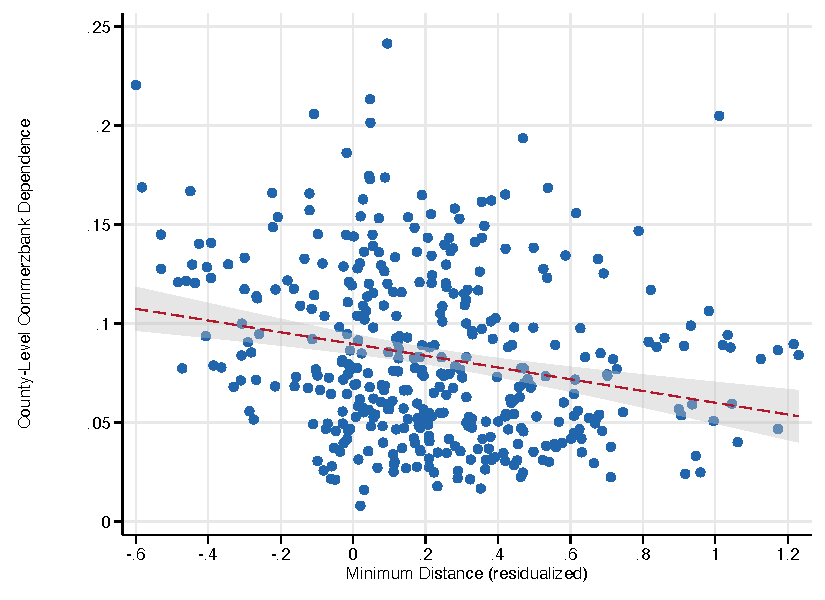
\includegraphics[width=1\linewidth]{first_stage_graph}
    \begin{tablenotes}
        \footnotesize
        \item \textbf{Note:} The graph shows the relationship of the exposure to the credit shock at county-level proxied by Commerzbank dependence and the county-level minimum geodesic distance from Commerzbank Headquarters in the Occupation Period from 1948 to 1957, residualized from an indicator variable indicating that the county was in East Germany, the single distances from Post-WWII headquarters, and the distance from Berlin and Dresden, former pre-war head offices.
    \end{tablenotes} 
\end{figure}

However, plotting the reduced form using $\delta$(Populist Party Support 2007-2012), defined as $\ln$(average populist party support in 2012 + 1) - $\ln$(average populist party support in 2007 + 1), where the average populist party support is measured at county level using the answers to the SOEP questionnaire, we find no relationship with our measure of Commerzbank relationship, in contrast with \citet{bib:huber2018}. We should try to \hl{plot the reduced form for county GDP growth 2007-2012 to understand whether we are doing something wrong with respect to what Huber does}. Trying to run the 2SLS with the main specification and using $\min\parens{Distance} \times Post$ as instrument, keeping the two-way fixed effects, we obtain negative point estimates and big standard errors, as described in Table \ref{tab:secondstage}.

\begin{table}[hbtp!]
\centering
\caption{The Effect of the Credit Shock on Political Preferences: Trying out IV Estimates}\label{tab:secondstage}
%\def\sym####1{\ifmmode^{####1}\else\(^{####1}\)\fi}
\resizebox{.6\textwidth}{!}{%
\begin{tabular}{lccc}
\toprule
& \multicolumn{1}{c}{(1)}
& \multicolumn{1}{c}{(2)}
& \multicolumn{1}{c}{(3)}
\\ 
\midrule
$ Exposure_{k}\ \times \ Post $&  -0.010\tsup{*}  &      -0.007         &      -0.007\\
           &     (0.006)         &     (0.005)         &     (0.005)\\
$ \min(Distance)_{k}\ \times \ Post $&       0.889\tsup{***}&       0.883\tsup{***}&       0.881\tsup{***}\\
           &(0.165)         &     (0.162)         &(0.161)         \\
\\
Number of Observations&229,699         &     206,604         &     206,604\\
Adjusted $ R $-Squared&       0.012         &       0.014         &       0.014\\
Kleibergen-Paap $ F $-Statistic&       28.88         &       29.79         &       30.00\\
Number of Counties&         396         &         396    &         396         \\
\midrule
County-Level FE&         Yes         &         Yes         &         Yes         \\
Wave FE&         Yes         &         Yes   &         Yes         \\
Basic Controls&         Yes         &         Yes &         Yes         \\
Household Controls&          No         &         Yes         &         Yes         \\
Regional Controls&          No         &          No         &         Yes         \\
\bottomrule
\end{tabular}
}%
\caption*{\footnotesize \textbf{Notes:}~This table shows the 2SLS estimates from \eqref{eq:twfecurrent}, instrumenting the measure of exposure to the credit shock at county level with the (negawtive) minimum geodesic distance of the county from the Post World War II Headquarters of Commerzbank.}
\end{table}

We have been trying to understanding why the standard errors turn so big: this is either because the OLS estimates are truly upward biased, or because we have no variation left to exploit given the nature of the dependent variable. What we are trying to estimate is a LATE on the compliers, but we might have a lot of counties where there is no variation for many reasons. We can try to look at test on descriptives taking conditional means of the population to see how they differ and why they are eating out the variation. With 395 counties in total, of which 75 are in East Germany and 320 in West Germany, calculating populist party support from 2007 to 2012 as

\begin{align*}
    \Delta\parens{\text{Populist Party Support 2012-2007}}_{k} &= \\
    &\ln\parens{1 + \frac{1}{N_{k}^{2012}}\sum_{i \in N_{k}^{2012}} \ind{Populist}_{ik}^{2012}}\\
    &- \ln\parens{1 + \frac{1}{N_{k}^{2007}}\sum_{i \in N_{k}^{2007}} \ind{Populist}_{ik}^{2007}}
\end{align*}

we obtain:

\begin{itemize}
    \item 209 counties with zero variation, because either there is no variation of there is no variation in the sample, 203 of which are in West Germany and 6 in East Germany;
    \item 74 counties with increase of share in intention to vote for a populist party, 39 of which are in West Germany and 35 in East Germany;
    \item 112 counties with decrease of share in intention to vote for a populist party, 78 of which are in West Germany and 34 in East Germany.
\end{itemize}

What does it mean? Most of the counties have zero variation, so it might be possible that there is not enough power in the representative sample. Increasing observations with the repeated cross-sections, it might give more variation at the level of these counties.


% Supply-Side Response
%-----------------------------------------------------------------------------

\section{Supply-Side Response to Shifts in Populism Demand}

\subsection{Text Analysis Improvements}

\subsection{Effect Decomposition}

% Miscellaneous
%-----------------------------------------------------------------------------

\section{Miscellaneous}

% \input{\TablesPath table_3.tex}

%-----------------------------------------------------------------------------------
% \begin{figure}[H]
%     \caption{The growth of the broad money and inflation during 2010Q1--2021Q2}
%     \label{fig:2}
%     \begin{subfigure}[b]{0.5\linewidth}
%         \caption*{Panel A: Broad Money} \vspace{-.5em}
%         \label{fig:2a}
%         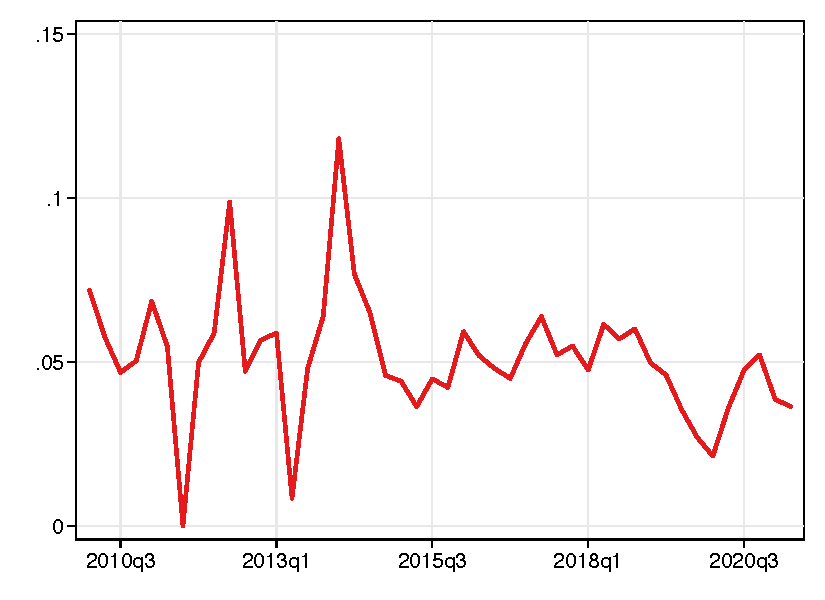
\includegraphics[width=1\linewidth]{moving_m2} 
%     \end{subfigure}%
%     \hfil
%     \begin{subfigure}[b]{0.5\linewidth}
%         \caption*{Panel B: Inflation} \vspace{-.5em}
%         \label{fig:2b}
%         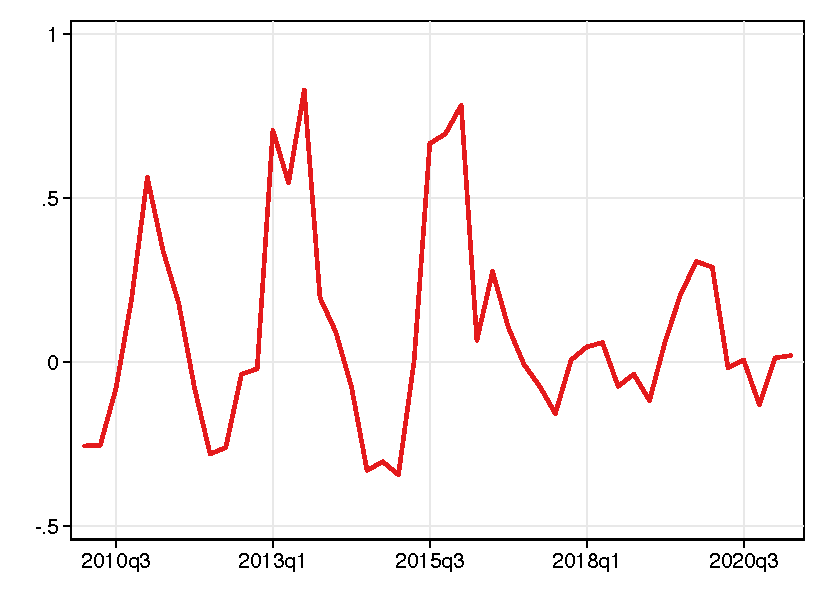
\includegraphics[width=1\linewidth]{moving_inflation}
%     \end{subfigure}
%     \begin{tablenotes}
%         \footnotesize
%         \item \textbf{Note:} This two figures represent the moving average of the broad money and inflation between 2010Q1--2021Q2. Panel A reports the broad money and Panel B reports inflation rate growth. The $y$-axis reports the percentage change with multiply by 100 bias, the $x$-axis is the time period in quarters. The data uses to plot these figure come the National Bank of Cambodia and the National Institute of Statistics.  
%     \end{tablenotes} 
%     
% \end{figure}

%----------------------------------------------------------------------------- %
%   References                                                                 %
%----------------------------------------------------------------------------- %

\clearpage\newpage
\bibliographystyle{aea}
\bibliography{../references/CreditPopulismReferences,../references/ExternalReferences}
% \printbibliography

\end{document}
